\chapter{Databases}

\pagestyle{fancy}

Databases are used in all disciplines in which an efficient data handling is needed, specially if those data are large. The data that are used in GIS are usually rather large, and the improvements in data acquisition have caused geographical data to be now more precise and, consequently, larger. 

Databases not only have the advantage of being able to work with large datasets, but also other ones such as managing multiple users or providing efficient access and indexing. For this reasons, they are a fundamental element in any software context, including GIS.

A \textbf{database} is an \textbf{organized and systematically stored collection of data}. Databases provide a better way of handling and using data, thanks to their structure.

Some of the advantages of using a database instead of a traditional file-based approach for storing data are:

\begin{itemize}
	\item \textbf{More independence}. Data are independent from both the users and the software.
	\item \textbf{More availability}. Databases facilitate the access to data from different contexts and applications, making them more useful for a larger number of users.
	\item \textbf{More security (data protection)}. Replication and synchronization of data becomes easier.
	\item \textbf{Less redundancy}. Which implies a smaller volume of data and faster access.
	\item \textbf{More efficiency in data capture, encoding and input}.
\end{itemize}

This has a direct influence in the results that are obtained from the exploitation of database data, and we find the following advantages:

\begin{itemize}
	\item \textbf{More coherence}. Better management leads to better data, and that produces results with a better quality.
	\item \textbf{More efficiency}. Accessing the data is easier and more effective.
	\item \textbf{More informative value}. It is easier to extract the information that is contained in the data, since one of the goals of a database is the increase the value of data as source of information.
\end{itemize}

Users also get advantages when using a database, such as the following ones:

\begin{itemize}
	\item \textbf{Easier access}. The user of the database just has to worry about \emph{using} the data. A solid infrastructure to do it is available, and so are the tools needed for it.
	\item \textbf{Easier data reutilization}. Data is easier to share when using a database.
\end{itemize}

In short, we can say that the main characteristic of a database is the \textbf{centralization} of data that it implies, which results in a \textbf{better data access, management and organization}.


\section{Relational databases}

From the many different models that have been defined for creating a database, the most popular one, both in the GIS context and outside of it, is the one used in databases known as \textbf{relational databases}. This model uses a scheme based on \textbf{tables}, which is both easy to understand and to use for analysis and data queries. Tables have a certain number of \textbf{records} (rows) and \textbf{fields} (columns).

The table itself is knows as a \textbf{relation}, since it contains the relation that exists between its elements. Columns represent the \textbf{attributes} associated to a feature, while rows contain the \textbf{records}. A row is formed with a set of $n$ attributes, which form a \textbf{tuple}.

A database usually contains more than a table, since the information to store is of many different types, and it is convenient to separate it into several tables. Apart from the relations that the table itself implies, relations between tables can also be defined. This is commonly know as a table \textbf{join}. To perform a table join, we need to have some attribute that can be used to unequivocally represent a tuple. This attribute is known as a \textbf{key attribute}, and it must be \textbf{unique and invariable} for each tuple. For instance, if we have a table where each row represents a person, an attribute containing the Social Security number can be used as a key attribute.

When working with geographical data, it is common to use \textbf{the spatial component as key}, since it is usually unique.

Relations between tables can be of several types, depending on the records of one table that are related with the ones of the other table. We have \textbf{one to one}, \textbf{one to many} and \textbf{many to many} relations. For instance, if we have a table with cities and another one with persons, and we define a relation \emph{lives in}, it will be a one to many relation, since many people can live in a a single city, and each person lives in only one of them.


\section{Database management systems}

Along with databases, the fundamental element to exploit them are \textbf{database management systems} (DBMS). These systems are an \textbf{intermediary element between the data and the software that consumes them}. Software such as a desktop GIS does not access the database directly, but instead \textbf{through a DBMS}.

The following are some of the characteristics that a DBMS must have:

\begin{itemize}
	\item \textbf{Transparent access to data}. The DBMS creates an abstraction of the data that makes it easier to work with them, hiding the internal elements that are not relevant for exploiting the data.

	Procedures such as \textbf{queries} are done through a DBMS, which takes care of interpreting them, applying them on the database and returning the corresponding result. The GIS does not query the database, but instead communicates with the DBMS.
	\item \textbf{Data protection}. If the database contains sensible information, a DBMS must \textbf{control the access to it}, restricting it to certain users and implementing the protection mechanisms that are needed for this.
	\item \textbf{Efficiency}. A DBMS must be capable of efficiently handling \textbf{a large volume of data and a large number of operations} (for instance, many users accessing simultaneously), and provide a quick response to user requests.
	\item \textbf{Transaction management}. Operations on a database such as adding or deleting a record are performed using what is known as a \textbf{transaction}. A transaction is a unit of work performed within a database management system against a database. A DBMS is said to be \textbf{transactional} if it can guarantee the integrity of the data and does not allow transactions to remain uncompleted. 

\end{itemize}

Since software such as a GIS communicates with the DBMS and does not access the database directly, a language to establish this communication is needed. Languages used to make queries to a DBMS are known as \textbf{query languages}. The most popular of these languages is the \textbf{Structured Query Language (SQL)}.

\subsection{Spatial databases}

We have seen the fundamental ideas about general databases, which can contain any type of data. Adding spatial data to this is not trivial, as it adds more complexity and makes it necessary to use a different approach. For a database to be considered spatial, it should be adapted to the particular nature of spatial data, and include additional elements.

First, the database has to be able to \textbf{store spatial data natively}. That means that a geometry can be stored in the table, just like it happens with other data types that can be used for table attributes, such as numerical values or text strings. Not only the database must be able to store spatial data, but also to \textbf{understand it} and be aware of its properties, so it can support queries related to that data. 

This is what makes the database fully spatially enabled, unlike a storage mechanism in which the geometry is stored using some of the basic data types (for instance, using a string containing the geometry coordinates), and the database does not know about its spatial nature (it makes no difference between that string and any other containing other type of information).

Although raster data can be stored as well, \textbf{spatial databases work mostly with vector data} and are better adapted to them. The geometries are stored as part of the attributes of a table record, which corresponds to a feature in the vector representation model. The thematic component can be stored in the database without requiring further adaptation.

Assuming that the database is prepared to store spatial data and correctly work with it, we now need to \textbf{adapt the query language}. Along with the usual operations that a DBMS can perform, new ones are added that use the spatial properties of spatial data. A query language that supports queries related to the spatial component of the data is known as a \textbf{spatial query language} .


\section{Queries}

A query is an operation in which we \emph{ask} the geographical data about the information they content. This type of analysis is one of the key elements of GIS, since it represents a large part of the work that is done with a GIS software.

Although queries are not exclusive of databases, they become more powerful and efficient with the help of a DBMS and a query language.

In the context of GIS, a query represents something similar to what we do when we use a classic paper map and, based on it, we respond to questions such as \emph{which is the closest river to X city?} or \emph{which rivers cross the Y province?}. We must not forget, however, that geographical data has two components: a thematic one and a spatial one. Questions such as the ones above refer only to the spatial component, but we can make queries that refer to the thematic one, or, moreover, to both of them simultaneously.

A very simple example of a query is \textbf{selection}. This is an operation that is commonly performed in a GIS, to just work with a subset of all the features in a layer. In figure \ref{Fig:Selection} you see how the GIS user defines a rectangular area, and features that fall within its limits are selected. Selection criteria can be as simple as this one, or more complex, and they might also include the thematic component (here we are just using the spatial one).

\begin{figure}[!hbt]   
\centering
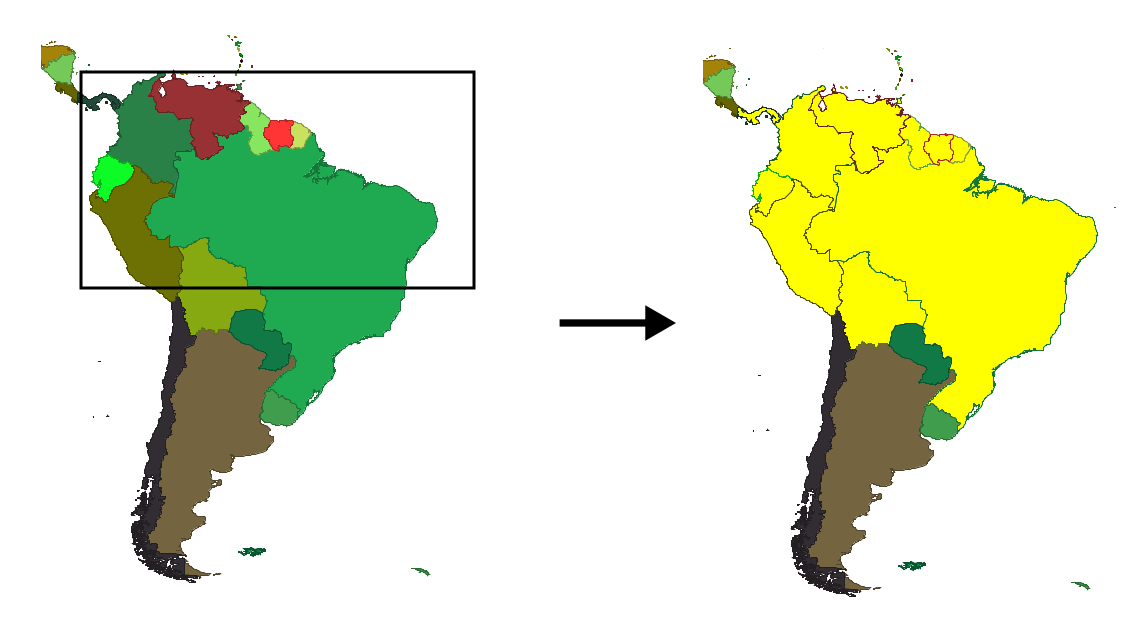
\includegraphics[width=\textwidth]{databases/Selection.png}
\caption{\small Manual selection of features by defining a rectangular region.}
\label{Fig:Selection} 
\end{figure}


A query can also be used to extract certain information from a database according to our needs, and to later create a new layer with it. This operation is very useful when the database contains a large amount of data, but we only need a part of those data. We might create a subset based on spatial criteria (for instance, if the database contains information for the whole world and we just want the one corresponding to a given country), a thematic one (the database contains many attributes associated to each feature, but only a few of them are of interest to us), or a combination of both. To extract that information and create a subset of the original data, we will use a query.

Let's see some more examples of queries. Let's assume that we have a layer with the world countries, and a set of economic and social parameters associated to each of them. For each country, we also have a polygon representing its boundaries.

We can make queries like the following ones:

\begin{itemize}
 \item Which countries have a GDP larger that Spain's one?
\item Which countries have grown economically during the last year?
\item Which countries have a population of more than 200 million people? 
\end{itemize}

In this queries, we are not using the spatial component (we do not need the polygon associated to each country). We could make those queries if we had country data without any spatial component, and using a regular database with no spatial capabilities.

Queries might include several criteria. For instance:

\begin{itemize}
 \item Which countries that have grown economically during the last year have a population of more than 40 million people?
\item In which countries where English is spoken population increased during the last year?
\end{itemize}

To express this queries in a way that can be later adapted to a query language, we need to use \textbf{logical operators}. The above queries would be rewritten as follows.

\begin{itemize}
 \item Which countries have grown economically during the last year \emph{and} have a population of more than 40 million people?
\item In which countries is English spoken \emph{and} the population increased during the last year?
\end{itemize}

Query languages that can be used to communicate with a DMBS support these operators for queries.

If the DBMS is spatial and \emph{understands} that certain columns of a table contain spatial information, it will support queries that use that information, such as the following ones:

\begin{itemize}
\item Which country spans the most degrees of latitude?
\item How many countries are completely contained in the southern hemisphere?
\item Which countries are located at less than 2000 km from Spain?
\end{itemize}

To respond to these queries, we just need to analyze the spatial component, and we do not need the rest of the attributes data. These queries are purely spatial. Although they extend what we had done before, we are not adding here any new way of studying geographical data that was not possible without a GIS. We could respond to those queries using just a classic paper map.

The true power of spatial queries is to allow querying both the thematic and the spatial component. For instance, with queries such as these:

\begin{itemize}
 \item Which countries in the southern hemisphere have a population density higher than the one of Peru?
\item How many countries with a population of more than 10 million people share their borders with Russia?
\end{itemize}

These queries require analyzing the thematic component, and at the same time include criteria that are based on the spatial and topological relations of the associated geometries.

Queries can include \textbf{several layers}. For instance, if along with the countries layer that we have been using, we have a layer with rivers, we could respond to a query such as \emph{Which countries does the Nile river cross?}. This is a purely spatial query that uses two layers.

Table joins, which were discussed for regular databases with no spatial data, can also be performed with a spatial criteria. These are known as \textbf{spatial joins}.

Here is an example of a spatial join. Suppose that we have a layer with world cities and the layer with countries that we have been using in previous examples. We can define a relation between the two corresponding tables, which will associate to each city all the attributes of the country it belongs to. A field with the country name in both tables is needed for that, to use it as the linking point. 

However, even if we do not have such a field, we can join the tables if we have spatial data for both cities and countries. All cities that belong to a given country must be located within its boundaries. This can be used to define the relation between the tables, and we can know which country a city belongs to, just by finding the polygon from the countries list in which the point representing the city is located.


\subsection{Spatial indexes}

If we make a query to a spatial database, responding to it might involve a large number of operations. If, using our countries layer, we want to know which countries have a population of more than 10 million people, we need to read the population of every single country in our table and compare it to that value. If the table has a large number or records, the query might take long to be processed. We can clearly see that this is not the optimal way of processing a query.

By using what is known as \textbf{indexes}, we can reach the data that will form the response of our query in a shorter time, without having to pass through all the data contained in the database.

This is easy to understand with an example. Imagine a telephone book. It contains a large number of entries, but you can easily find a name without having to read them all. This is because a) the data is ordered (\textbf{indexed}) in a particular way (alphabetically) and b) you know how to use that indexing (you know the order of letters in the alphabet). With that, you know that it does not make sense to search for a certain Mr. Johnson in the pages that correspond to letter A or B, and you can skip them.  

Apart from indexes for numerical or alphanumerical values, which are easy to create, another type of indexes, known as \textbf{spatial indexes}, are of great importance in the context of GIS. The concept is similar to non-spatial indexes, and serve the same purpose: to \textbf{optimize searches using a correct data structure}, in this case based on its spatial component.

We will use another example to help understand how an spatial index works. Suppose that we are using our layer with countries and the want to find those that are located at less than 2000 km from Spain. How would we proceed to response to this query? 

A naive approach would be to measure the distance between Spain and all the remaining countries, then select those at a distance of less than 2000 km. We would get the correct result, but this approach is far from optimal. 

Finding a better approach is easy. For instance, with a little knowledge of world geography, we can immediately exclude all countries in America. We can be sure that they will not be part of the response, since the distance between Spain and America is already larger than 2000 km. We do not know the distance between those countries and Spain, but we are sure that it will be more than 2000 km. Therefore, it makes no sense to measure the distances to all of them.

That knowledge of world geography that allows us to reduce the number of countries to work with is actually like a spatial index. It cannot be used to respond to the query, but it \textbf{provides an approximation that makes it easier to respond to it}. We can discard a large number of countries, and then perform the most costly operations (the measurement) with just a subset.

Thanks to spatial indexes, queries are more efficient and we can work with larger datasets.

Indexes (both spatial and non-spatial ones) are stored along with the data they refer to, whether in separate files or inside the database itself. Spatial DBMS have \textbf{built-in capabilities to compute those indexes} and store them, and once they have been computed, they are used whenever the DBMS has to respond to a spatial query.


\pagestyle{empty}
